\documentclass[dvipdfmx]{beamer}
\usepackage{pxjahyper}
\usepackage{bookmark}
\usepackage{txfonts}

\usetheme{Copenhagen}
\usecolortheme{rose}

\renewcommand{\familydefault}{\sfdefault}
\renewcommand{\kanjifamilydefault}{\gtdefault}

\renewcommand{\figurename}{図}
\renewcommand{\tablename}{表}

\setbeamercovered{dynamic}

\setbeamertemplate{headline}{}
\setbeamertemplate{footline}[page number]
\setbeamertemplate{navigation symbols}{}
\setbeamertemplate{section in toc}[sections numbered]
\setbeamertemplate{items}[default]
\setbeamertemplate{blocks}[rounded]

\usefonttheme{professionalfonts}
\usefonttheme[onlymath]{serif}
\usefonttheme{structurebold}
\setbeamerfont{frametitle}{size=\Large}
\setbeamerfont{title}{size=\Large}

\title{3. 画像のループバック}
\author{201720690 小松 弘人}
\date{\today}

\begin{document}

\maketitle

\begin{frame}
	\frametitle{Agenda}
	\tableofcontents
\end{frame}

\section{演習目的}
\begin{frame}
	\frametitle{演習目的}
	\begin{itemize}
		\item
			本演習の進め方を理解する
			\vfill
		\item
			FIFOの基礎を実践しながら理解する
	\end{itemize}
\end{frame}

\section{演習概要}
\begin{frame}
	\frametitle{演習概要}
	\begin{enumerate}
		\item
			Vivadoで画像をそのまま戻す回路を記述
			\vfill
		\item
			Xillinux起動用SDカードを準備
			\vfill
		\item
			実機で動作を確認
	\end{enumerate}
\end{frame}

\section{事前準備}
\begin{frame}
	\frametitle{vivadoでxillydemoプロジェクトを作成する (windows)}
	\begin{enumerate}
		\item
			xillinuxリポジトリをダウンロードする
			\vfill
		\item
			Vivadoを起動
			\vfill
		\item
			Tools→Run Tcl Script...でverilog/xillydemo-vivado.tcl実行
	\end{enumerate}
\end{frame}

\begin{frame}[fragile]
	\frametitle{Xillinuxのブート用SDカードを作成する (Linux版)}
	\begin{enumerate}
		\item
			公式ページからSDカードイメージをダウンロード
			\vfill
		\item
			xillinux-1.3.img.gzを解凍
			\vfill
		\item
			\verb|dd|でSDカードに書き込む
			\vfill
		\item
			SDカードの1つ目のパーティションにファイルをコピー
			\vfill
		\item
			SDカードの1つ目のパーティションにxillydemo.bitをコピー
	\end{enumerate}
\end{frame}

\begin{frame}[fragile]
	\frametitle{Xillinuxの環境設定・事前準備 (Xillinux)}
	\verb|startx|でGUIが起動できる\\
	GUIは必須ではないが、GUIで演習を進めることを勧める

	\begin{itemize}
		\item
			キーボードの設定
			\vfill
		\item
			IPアドレスの設定
			\vfill
		\item
			\verb|apt-get|で\verb|git|, \verb|g++|,
			\verb|openssh-server|のインストール
			\vfill
		\item
			\verb|passwd|でパスワードを設定
	\end{itemize}
\end{frame}

\section{演習 (Windows)}
\begin{frame}
	\frametitle{演習内容}
	\begin{enumerate}
		\item
			Vivadoでxillydemoプロジェクトを開く
			\vfill
		\item
			loopback.vをプロジェクトに追加する\\
			入出力ポートはFIFOと同じ
			\vfill
		\item
			wrapper.vを編集し、loopbackを追加する
			\vfill
		\item
			loopback.vを編集する
	\end{enumerate}
\end{frame}

\begin{frame}
	\frametitle{loopbackモジュール}
	\begin{figure}[ht]
		\centering
		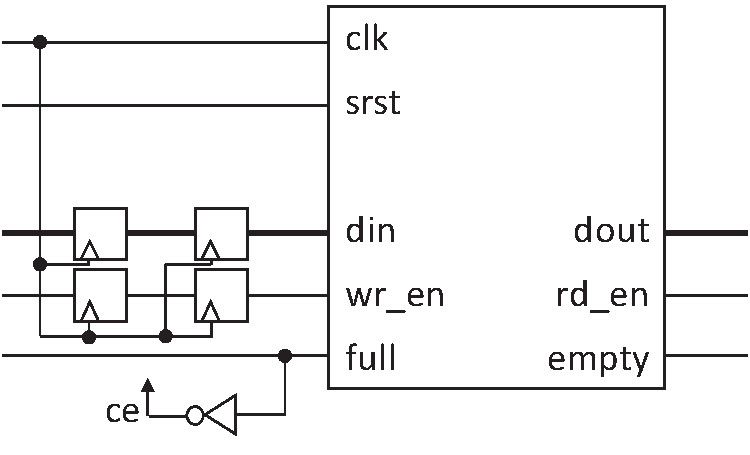
\includegraphics[width=0.8\linewidth]{../img/loopback.pdf}
		\caption{ブロック図}
		\label{img:loopback}
	\end{figure}
\end{frame}

\section{演習 (Xillinux)}
\begin{frame}[fragile]
	\frametitle{演習用プログラムの実行 (Xillinux)}
	\begin{itemize}
		\item
			Xillinux上でsoftwareリポジトリをダウンロード
		\item
			そのディレクトリでmakeを実行
	\end{itemize}
	プログラムは\verb|bin/send_bmp src.bmp dst.bmp|のように実行する
\end{frame}

\section{出力画像の確認}
\begin{frame}
	\frametitle{出力画像の確認}
	\begin{itemize}
		\item
			出力画像→入力画像をグレースケールにした画像になるはず
			\vfill
		\item
			Xillinuxのディスプレイは各色$4\mathrm{[bit]}$
			なのでWindows上で確認すること
	\end{itemize}
\end{frame}

\end{document}
